% !TEX root = mythesis.tex

%==============================================================================
\chapter{Theoretical concepts}
\label{chap:theory}

This chapter provides a brief introduction of the standard model of particle physics. A brief introduction of top quark physics which is crucial for analysis in this thesis, is also presented in this chapter.

\section{The standard model of particle physics}

The standard model of particle physics (SM) is the theory describing three of the four known fundamental forces in the universe, as well as classifying all known elementary particles. The fundamental forces explained by SM are electromagnetic, weak and strong interactions, while omitting gravity. The SM is a gauge theory of quantum fields, a mathematical framework combining classical field theory, special relativity and quantum mechanics. It utilizes a Lagrangian in order to describe the dynamics of the quantum state and fundamental fields. This Lagrangian is invariant under SU(3)$_{C}$\times SU(2)$_{L}$\times U(1)$_{Y}$ symmetry group \cite{Peskin:1995ev}. The strong interaction is represented by the SU(3)$_{C}$ group, while the unified electroweak interaction is represented by the SU(2)$_{L}$\times U(1)$_{Y}$ group.  \\

\begin{figure}[!h]
\centering
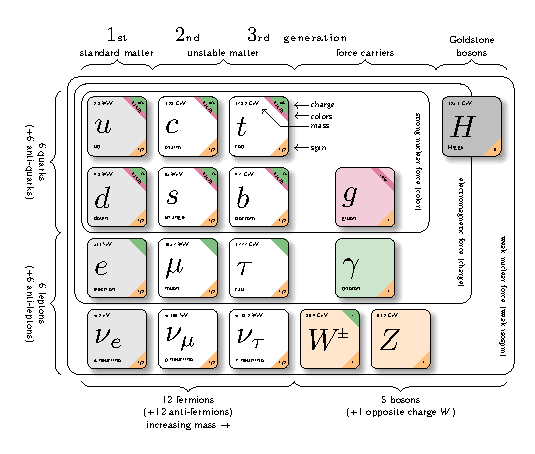
\includegraphics[width=0.83\textwidth]{ubonn-thesis/Chapters/Chapters_02/Figure/Standard_Model.pdf}
\caption{Standard Model of Particle Physics \cite{sm}}
\label{standardmodel}
\end{figure}

Each force operates on a different on a different range and with different strengths. The strong and weak forces are very limited range and dominate only on the level of subatomic interactions, while electromagnetic forces have infinite range. The SM consists of 17 fundamental particles classified into two groups: half-integer spin fermions, and integer spin bosons. The spin-1 (vector) bosons act as the mediators of interaction between particles and the spin-0 (scalar) Higgs boson acts as the mediator of Higgs interactions. An illustration of SM particles with their mass, charge and spin is presented in figure \ref{standardmodel}.



\subsection{Fermions}
There are 12 spin-$\frac{1}{2}$ fermions in the SM: 6 quarks and 6 leptons, which are grouped into 3 generations which are grouped into 3 generations. Each generation of quark contains one quark of charge +2/3e (up-type) and one quark of charge -1/3e (down-type). The quarks are (up-type followed by down-type): up (u) and down (d); charm (c) and strange (s); and top (t) and bottom (b). Similarly three lepton generations consists of electron (e), muon ($\mu$), and tau ($\tau$), and their corresponding neutrinos ($\nu_{e}$, $\nu_{\mu}$, $\nu_{\tau}$). The neutrinos have no electric charge, while the other leptons carry an electric charge of -1e. Each fermion has its corresponding anti-particle, with opposite sign on all charges (such as electric charge \& quantum numbers) but identical mass.

In the SM, a quark of one flavor can transform into a quark of another flavor via weak interaction. It strongly prefer to transform into another quark of its same generation. The transformation probability scale with the couplings in the Cabibbo-Kobayashi-Masakawa (CKM) matrix. For more details ref. \cite{Bargiotti:2000dn} can be referred.

\subsection{Bosons}

The remaining five particles in the SM are comprised of four vector type (spin-1) boson and one scalar type (spin-0) Higgs boson. Apart from the Higgs boson, all other bosons are called gauge bosons and are the mediators of the fundamental interactions between particles. Photons are the mediators of the electromagnetic force and are massless. The massive W and Z bosons   ($m_{W}$ = 80.379 GeV, $m_{Z}$ = 91.1876 GeV) are the mediators of the weak force while strong force is mediated by massless gluons. The gluons as well as quarks carry colour charge. There are three different colour charges: red, green, and blue. Additionally, there are also three anticolours (for antiparticles). Gluons themselves carry a combination of a colour and an anticolour charge and therefore they can couple to each other. There are only eight gluons in total because one of the nine colour combinations results in a non-existing colour singlet state. 

%\section{Physics at hadron colliders}

\section{Top quark physics}
The neutral Kaon decays experiment in 1964 by Christenson, Cronin, Fitch, and Turlay showed that weak interaction is not invariant under the combined discrete symmetry operation of charge conjugation C and parity P (CP violation) \cite{PhysRevLett.13.138}. Kobayashi and Maskawa realized that SM can provide a mechansim of CP violation through flavor mixing only if there are at least three generation of quarks \cite{kobayashi1973cp}. After the discovery of bottom quark in 1977 in Fermilab \cite{PhysRevLett.39.252}, the existence of the top quark as the weak isospin was expected. The top quark was first observed at the D0 and CDF collaborations on the Tevatron in $p\Bar{p}$ collisions in 1995 \cite{PhysRevLett.74.2626,PhysRevLett.74.2632}. Nowadays LHC is a top quark factory where top quarks are produced as discussed in section \ref{subsec:topquarkproduction}  .

\subsection{Top quark}
\label{subsec:topquark}
The top quark is the heaviest fundamental particle in the SM. It is up-type third generation quark. It has an electric charge Q = $\frac{2}{3}$, a mass of 173.3 $GeV/c^{2}$ and a decay width of $\Gamma_{t}(\alpha_{s}(M_{Z}) = 0.118)=$ 1.35 $GeV/c^{2}$ which corresponds to an average lifetime of $\tau_{t} \approx 0.5 \times 10^{-24}$ s \cite{ParticleDataGroup:2016lqr}. The top quark exclusively decays via weak interaction before hadronization, producing a W boson and a bottom quark because of its extremely short-lived lifetime. The absence of a hadron surrounding the top quark produces physicists with the unique opportunity to study the behaviour of a "bare" quark.

\subsection{Top quark production}
\label{subsec:topquarkproduction}

Top quarks are  dominantly produced in pairs through quark anti-quark annihilation and gluon-gluon fusion at leading order in QCD at haron colliders such as Tevatron and LHC. They are also produced singly through electroweak processes. At the LHC, top-quarks are mainly produced via gluon-gluon fusion. In this production mechanism two gluons from protons fuse into another gluon (see figures \ref{fig:gg1} and \ref{fig:gg2}) , or they exchange a virtual top quark and then emit a real $t\Bar{t}$ pair (see figure \ref{fig:vittt}). Figure \ref{fig:ttbarproduction} shows the leading order Feynman diagrams producing top anti-top pairs. 

\begin{figure}[h!] 
  \begin{subfigure}[b]{0.33\linewidth}
    \centering
    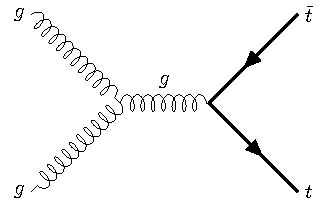
\includegraphics[width=\linewidth]{ubonn-thesis/Chapters/Chapters_02/Figure/ttbar_gluongluonchannel.pdf} 
  \caption{}
  \label{fig:gg1}
  \end{subfigure}%% 
  \begin{subfigure}[b]{0.33\linewidth}
    \centering
    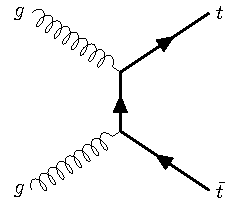
\includegraphics[width=0.76\linewidth]{ubonn-thesis/Chapters/Chapters_02/Figure/ttbar_Production_tchannel.pdf} 
  \caption{}
  \label{fig:gg2}
  \end{subfigure} 
  \begin{subfigure}[b]{0.33\linewidth}
    \centering
    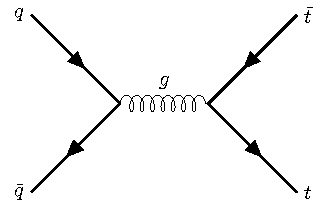
\includegraphics[width=\linewidth]{ubonn-thesis/Chapters/Chapters_02/Figure/ttbar_quarkquarkchannel.pdf} 
  \caption{}
  \label{fig:vittt}
  \end{subfigure}%%
  \caption{Leading order Feynman diagrams for $t\Bar{t}$ production via the strong interaction at the LHC}
  \label{fig:ttbarproduction}
  \end{figure}


Top quarks can also be produced singly in electroweak processes. The production processes are classified by the virtuality of the W boson exchanges in the process. The most abundant single top-quark production process at the LHC is t-channel production, followed by the associated production of a top quark and a real W boson, and s-channel production. Leading order diagrams of these processes are shown in figure \ref{fig:singletopproduction}. The production cross-section of these processes at LHC by the ATLAS colloboration is shown in figure \ref{ATLAS:singletop}. At the Tevatron, t-channel and s-channel single top-quark production are predicted by the SM, while Wt contribution is negligible \cite{singtop2014}.

\begin{figure}[h!] 
  \begin{subfigure}[b]{0.33\linewidth}
    \centering
    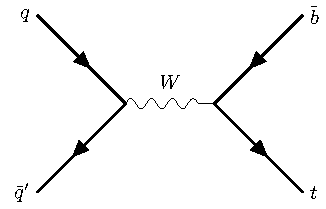
\includegraphics[width=0.96\linewidth]{ubonn-thesis/Chapters/Chapters_02/Figure/singletop_s-channel.pdf} 
  \caption{}
  \end{subfigure}%% 
  \begin{subfigure}[b]{0.33\linewidth}
    \centering
    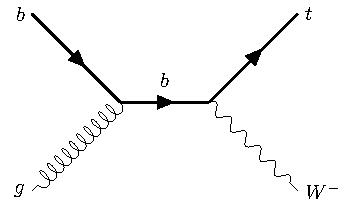
\includegraphics[width=\linewidth]{ubonn-thesis/Chapters/Chapters_02/Figure/singletop_realW.pdf} 
  \caption{}
  \end{subfigure} 
  \begin{subfigure}[b]{0.33\linewidth}
    \centering
    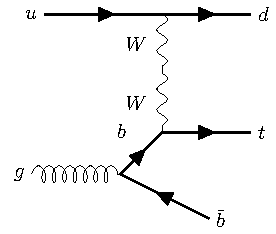
\includegraphics[width=0.76\linewidth]{ubonn-thesis/Chapters/Chapters_02/Figure/tchannel_4FS.pdf} 
  \caption{}
  \end{subfigure}%%
  \newline
  \centering
%  \vspace*{0.4cm}
  \begin{subfigure}[b]{0.4\linewidth}
    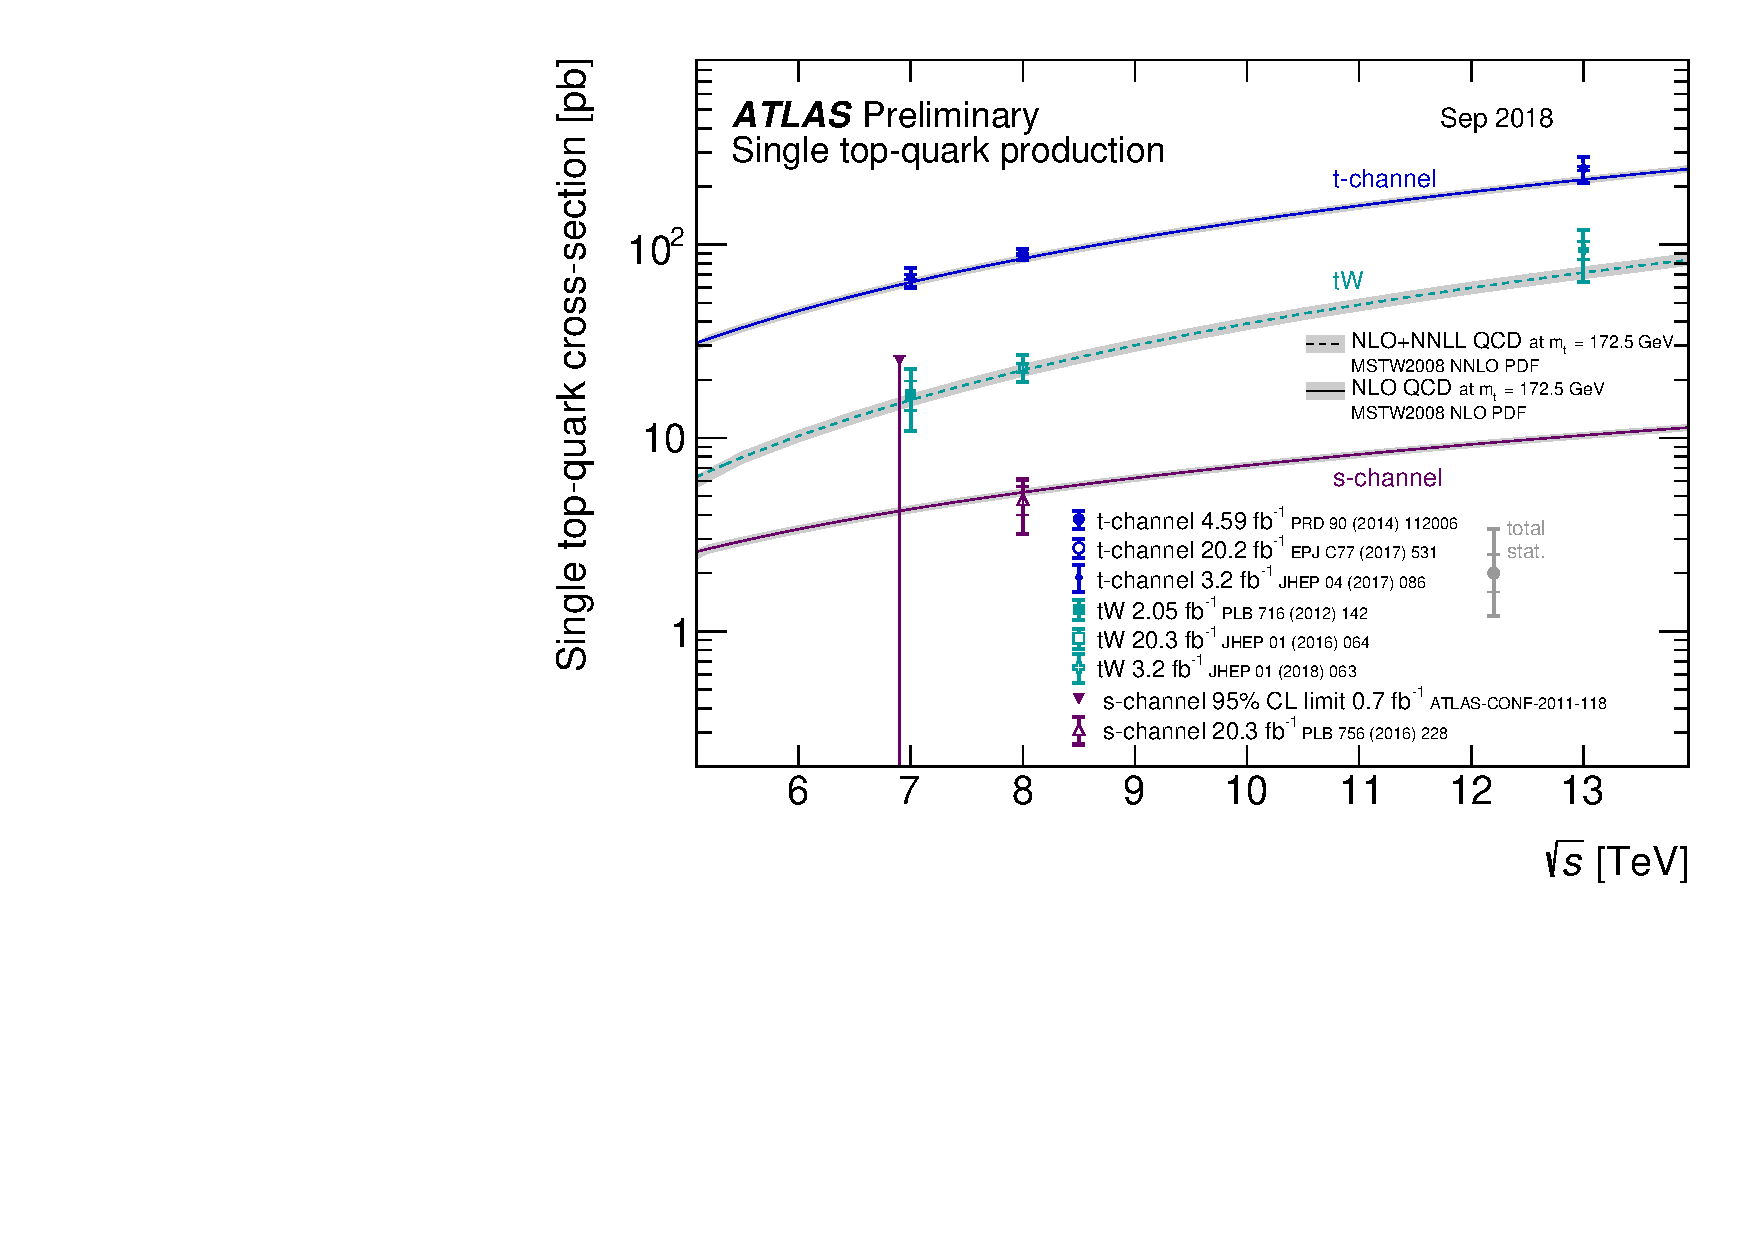
\includegraphics[width=\linewidth]{ubonn-thesis/Chapters/Chapters_02/Figure/singletop.pdf} 
  \caption{}
  \label{ATLAS:singletop}
  \end{subfigure}%%
  \caption{Feynman diagrams for single top quark production in the (a) s-channel, (b) in association with a W boson (c) t-channel production in 4FS , (d) measured single top quark production in ATLAS \cite{andrea}}
  \label{fig:singletopproduction}
  \end{figure}

By moving to next-to-leading order (NLO) electroweak production, there can be added to the single top processes, the radiation of a Z boson. This production process for which the total cross-section is measured in this thesis consists of a top quark, a forward-jet and a Z boson at the parton level. The top quark is produced via the t-channel and the Z boson is either radiated of from one of the participating quarks or produced via W boson fusion. The Feynman diagrams of the tZq process at the leading are shown in figure \ref{fig:tZQ}. As can be seen from figures \ref{topcoup} and \ref{wwzcoup}, tZq production offers access to the coupling of the top quark to a Z boson and additionally to the WWZ coupling. Measuring this process is therefore a very interesting test of the SM, since the production rate could be modified by several BSM theories (e.g. in vector-like quark models). 

\begin{figure}[h!] 
  \begin{subfigure}[b]{0.33\linewidth}
    \centering
    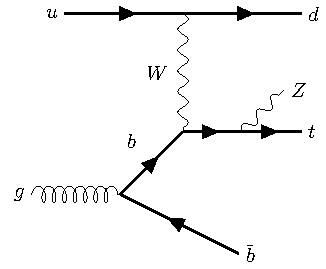
\includegraphics[width=0.7\linewidth]{ubonn-thesis/Chapters/Chapters_02/Figure/tZq_Zfromtop.pdf} 
  \caption{}
  \label{topcoup}
  \end{subfigure}%% 
  \begin{subfigure}[b]{0.33\linewidth}
    \centering
    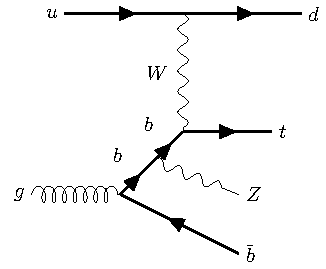
\includegraphics[width=0.7\linewidth]{ubonn-thesis/Chapters/Chapters_02/Figure/tZq_Zfromb.pdf} 
  \caption{}
  \end{subfigure} 
  \begin{subfigure}[b]{0.33\linewidth}
    \centering
    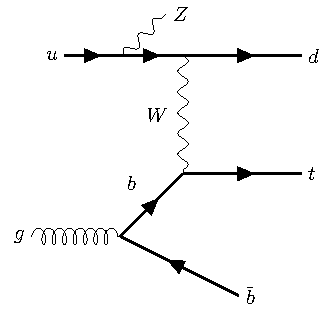
\includegraphics[width=0.7\linewidth]{ubonn-thesis/Chapters/Chapters_02/Figure/tZq_Zfromu.pdf} 
  \caption{}
  \end{subfigure}%%
  \newline
  \begin{subfigure}[b]{0.33\linewidth}
    \centering
    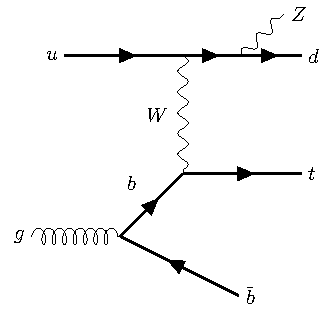
\includegraphics[width=0.7\linewidth]{ubonn-thesis/Chapters/Chapters_02/Figure/tZq_Zfromd.pdf} 
  \caption{}
  \end{subfigure}%% 
  \begin{subfigure}[b]{0.33\linewidth}
    \centering
    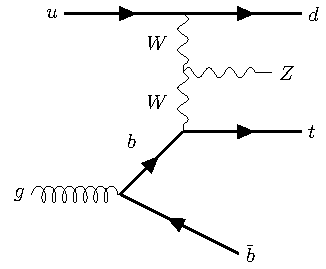
\includegraphics[width=0.7\linewidth]{ubonn-thesis/Chapters/Chapters_02/Figure/tZq_ZfromWW.pdf} 
  \caption{}
  \label{wwzcoup}
  \end{subfigure}
  \caption{Feynman graphs to calculate the lowest order amplitudes of the tZq process. In the four-flavour scheme, the b-quark originates from gluon splitting..}
  \label{fig:tZQ}
  \end{figure}